\documentclass[conference]{IEEEtran}
\usepackage{cite}
\usepackage{amsmath,amssymb}
\usepackage{graphicx}
\usepackage{booktabs}
\usepackage{url}
\usepackage{textcomp}
\def\BibTeX{{\rm B\kern-.05em{\sc i\kern-.025em b}\kern-.08em T\kern-.1667em\lower.7ex\hbox{E}\kern-.125em X}}

\begin{document}

\title{Deep Learning for Flight Delay Prediction: Entity-Embedding Networks, Ablations, Calibration and an Offline Rescheduling Study (Phase~2)}

\author{
\IEEEauthorblockN{[Member 1], [Member 2], [Member 3], [Member 4], [Member 5]}
\IEEEauthorblockA{Team ID: [T0XX] \\ Rishihood University, Sonipat, Haryana, India}
}

\maketitle

\begin{abstract}
We predict whether a US domestic flight will arrive at least 15 minutes late, using only information available two hours before scheduled departure. The data are the 327,346 labelled NYC flights of 2013, split strictly by time (70/15/15). Phase~1 used schedule-only features and reached a test PR~AUC of 0.308 with logistic regression. In Phase~2 we add seven leakage-tested history features and train a compact PyTorch MLP with learned embeddings for carrier, origin and destination, using dropout, weight decay, batch normalisation, class weighting and early stopping. The history features raise PR~AUC from 0.308 to 0.470 (logistic regression); the MLP reaches 0.472 (ROC~AUC 0.669), which is not distinguishable from logistic regression given a seed standard deviation of 0.005. Ablations show that the features matter far more than the architecture: embeddings do not beat one-hot encoding, and dropout, weight decay and embedding size change the score by less than two seed standard deviations. Calibration exposes a distribution shift: the delay rate is 15.4\% in validation but 26.7\% in test, so temperature scaling and Platt scaling fitted on validation make test calibration worse (ECE 0.041 $\rightarrow$ 0.072 and 0.117). An offline rescheduling simulation under explicit assumptions avoids 100--242 expected delays (1.0--2.4\% of all expected delays). We report these negative results openly.
\end{abstract}

\begin{IEEEkeywords}
flight delay prediction, deep learning, entity embeddings, probability calibration, temperature scaling, dataset shift, ablation study
\end{IEEEkeywords}

\section{Introduction}
Flight delays are costly for airlines, airports and passengers, and good predictions can support scheduling and passenger information \cite{carvalho}. This project predicts a binary outcome: will a flight arrive 15 or more minutes late? Two rules shape every design choice. First, the prediction is made two hours before the scheduled departure, so nothing that happens after that moment may be used. Second, the evaluation must respect time: models are trained on the past and tested on the future.

Phase~1 of the project built schedule-only features and compared logistic regression with gradient boosting. Its main weakness was weak signal (ROC~AUC about 0.57--0.60), because no information about recent delays at the airport was used. Phase~2, reported here, makes four contributions:
\begin{enumerate}
\item seven \emph{history features} built only from information known before the prediction time, with an automated leakage test;
\item a compact \emph{MLP with entity embeddings} and a regularisation recipe, compared fairly with logistic regression;
\item \emph{ablation studies} with a seed-noise estimate, so that we only claim differences larger than random variation;
\item a \emph{calibration} study and an \emph{offline rescheduling} what-if analysis with stated assumptions.
\end{enumerate}
We did not implement a hybrid or temporal model; the scope is deliberately limited to logistic regression versus an embedding MLP.

\section{Related Work and Deep Learning Literature}
\subsection{Flight delay prediction}
Rebollo and Balakrishnan \cite{rebollo} predicted departure delays 2--24 hours ahead with random forests, using the recent delay state of airports and of origin--destination links. Their key lesson, which we follow, is that \emph{recent delay state is the most informative signal}. Choi et al.\ \cite{choi} predicted weather-induced delays of individual flights with decision trees, random forests, AdaBoost and $k$-NN, and used sampling to handle imbalanced classes. Deep models then appeared: Kim et al.\ \cite{kim} modelled day-to-day delay sequences of an airport with LSTM networks and found that deeper recurrent architectures were more accurate; Yu et al.\ \cite{yu} combined a deep belief network with support vector regression on Beijing airport data; Yazdi et al.\ \cite{yazdi} used a stacked denoising autoencoder with Levenberg--Marquardt training on US flights. A systematic review \cite{carvalho} notes the rapid growth of machine-learning methods in this field. Most of these studies use richer inputs than ours (weather, network state, aircraft rotations).

\subsection{Deep learning on tabular data}
Our data are tabular, and deep learning is not automatically better here. Entity embeddings \cite{guoberk} map each category to a small learned vector and were designed for exactly this kind of data; they are the main deep-learning ingredient of our model. However, large benchmarks report that tree-based models often still outperform neural networks on typical tabular data \cite{grinsztajn}, and that deep models do not clearly beat simpler ones \cite{shwartz}. This sets a realistic expectation: a small MLP may only match a strong linear baseline, and our results confirm it.

\subsection{Regularisation and training}
Dropout \cite{srivastava} randomly removes units during training to prevent co-adaptation. Batch normalisation \cite{ioffe} stabilises the scale of hidden activations. AdamW \cite{adamw} decouples weight decay from the adaptive gradient step, which makes the penalty behave as true L2-style regularisation. Early stopping \cite{prechelt} halts training when validation performance stops improving. Class imbalance is commonly handled by re-weighting the loss \cite{johnson}, which we do with a positive-class weight.

\subsection{Evaluation and calibration}
For imbalanced problems the precision--recall curve is more informative than the ROC curve \cite{davis,saito}, so PR~AUC is our main metric. A model is \emph{calibrated} if its predicted probabilities match observed frequencies. Platt scaling \cite{platt} fits a logistic function on the model scores; Niculescu-Mizil and Caruana \cite{nm} compared such post-hoc methods. Guo et al.\ \cite{guo} showed that modern neural networks are often over-confident and that \emph{temperature scaling}, a single scalar fitted on validation data, is a simple and strong fix. The expected calibration error (ECE) \cite{naeini} and the Brier score \cite{brier} measure calibration quality. Importantly, Ovadia et al.\ \cite{ovadia} showed that calibration degrades under dataset shift, which is exactly what we observe.

\section{Data and Problem Setup}
\subsection{Dataset}
We use the 2013 NYC flights table (Kaggle), derived from US on-time performance data \cite{bts,wick}. It has 336,776 flights from EWR, JFK and LGA; 327,346 remain after removing flights without an arrival delay (e.g.\ cancelled). The target is $y=1$ if \texttt{arr\_delay} $\ge 15$ minutes. The overall delay rate is 24.5\%.

\subsection{Prediction time and leakage rules}
The prediction time is $T=\text{scheduled departure}-2\,\text{h}$. The flight's own \texttt{dep\_time}, \texttt{dep\_delay}, \texttt{arr\_time}, \texttt{arr\_delay} and \texttt{air\_time} are never used as inputs. Other flights' outcomes may be used only if they were already known at $T$.

\subsection{Chronological split}
Data are sorted by scheduled departure time and cut into train (70\%), validation (15\%) and test (15\%) without shuffling (Table~\ref{tab:split}). All scalers, encoders, imputation values, thresholds, temperatures and early-stopping decisions use training or validation data only; the test set is used once for reporting.

\begin{table}[t]
\caption{Chronological split and delay rate}
\label{tab:split}
\centering
\small
\begin{tabular}{lrcc}
\toprule
Split & Flights & Period (2013) & Delay rate\\
\midrule
Train & 229,142 & Jan 1 -- Sep 13 & 25.94\%\\
Validation & 49,102 & Sep 13 -- Nov 6 & 15.39\%\\
Test & 49,102 & Nov 6 -- Dec 31 & 26.69\%\\
\bottomrule
\end{tabular}
\end{table}

The delay rate is much lower in validation (autumn) than in train and test (summer storms, winter holidays). This shift is a property of one-year data and strongly affects thresholds and calibration (Section~\ref{sec:calib}).

\section{Feature Engineering}
Phase~1 features (16) are schedule, distance and cyclic time features (sine/cosine encodings of hour, weekday and month) plus carrier, origin and destination. Phase~2 adds seven history features (Table~\ref{tab:feat}), giving 20 numeric and 3 categorical inputs (23 features).

\begin{table}[t]
\caption{Phase~2 history features (all past-only)}
\label{tab:feat}
\centering
\small
\begin{tabular}{p{2.6cm}p{4.9cm}}
\toprule
Feature & Meaning\\
\midrule
origin delay rate, last 3\,h & Share of flights from the same origin that had already \emph{departed} before $T$ (within 3\,h) with $\ge$15 min departure delay\\
origin avg.\ dep.\ delay, 3\,h & Mean departure delay of those flights\\
origin delay rate, 24\,h & Same, over the last 24 hours\\
flights scheduled same hour & Number of scheduled departures from the origin in that hour (congestion proxy; the timetable is known in advance)\\
carrier history rate & Carrier's delay rate on \emph{earlier days} only\\
route history rate & Origin--destination delay rate on earlier days only\\
carrier--origin--hour rate & Same for carrier, origin and hour, earlier days only\\
\bottomrule
\end{tabular}
\end{table}

Missing values (for example on the first day of the year) are replaced by training-set means. The rolling features are computed with binary search and prefix sums, so any flight whose departure time is at or after $T$ is excluded by construction. An automated test changes the outcomes of same-day and future flights and checks that the features of earlier flights do not change; all three leakage tests pass. In the logistic regression, the strongest numeric coefficient is the 3-hour origin delay rate, in line with \cite{rebollo}.

\section{Methodology}
\subsection{Baseline}
Logistic regression with one-hot categories, standardised numeric features and balanced class weights is the baseline, trained on the Phase~1 and the Phase~2 feature sets.

\subsection{MLP with entity embeddings}
Carrier, origin and destination are mapped to integer ids (plus one out-of-vocabulary id) and to embeddings of size 4, 3 and 8. The embeddings are concatenated with the 20 standardised numeric features $\mathbf{x}$:
\begin{align}
\mathbf{h}_0 &= [\mathbf{e}_c;\mathbf{e}_o;\mathbf{e}_d;\mathbf{x}]\in\mathbb{R}^{35},\\
\mathbf{h}_1 &= \mathrm{Drop}_{0.3}\!\big(\mathrm{ReLU}(\mathrm{BN}(W_1\mathbf{h}_0+\mathbf{b}_1))\big),\\
\mathbf{h}_2 &= \mathrm{Drop}_{0.3}\!\big(\mathrm{ReLU}(W_2\mathbf{h}_1+\mathbf{b}_2)\big),\\
z &= \mathbf{w}_3^{\top}\mathbf{h}_2+b_3,\quad \hat p=\sigma(z),
\end{align}
with $W_1\in\mathbb{R}^{128\times35}$ and $W_2\in\mathbb{R}^{64\times128}$. The network has 14,097 parameters, of which 912 are embeddings. The architecture is small on purpose: with 229k training rows and only about 20 informative features, a larger network would mainly add variance. Embeddings let categories that behave alike share information, which a one-hot layer cannot do.

\subsection{Training and regularisation}
The loss is class-weighted binary cross-entropy,
\begin{equation}
\mathcal{L}=-\frac1N\sum_{i}\big[w_{+}\,y_i\log\hat p_i+(1-y_i)\log(1-\hat p_i)\big],
\end{equation}
with $w_+=N_-/N_+\approx 2.85$ from the training set. We use AdamW (learning rate $10^{-3}$, weight decay $10^{-4}$), batch size 1024, dropout 0.3, batch normalisation, and early stopping on validation PR~AUC (patience 5, at most 40 epochs, best weights restored). The seed is 42 unless stated. Training takes about 12 seconds on a CPU (PyTorch \cite{paszke}, scikit-learn \cite{sklearn}).

\subsection{Calibration}
\emph{Temperature scaling} \cite{guo} uses $\hat p=\sigma(z/T)$ with one scalar $T$ minimising the validation negative log-likelihood. \emph{Platt scaling} \cite{platt} fits a logistic regression on the model's log-odds. Both are fitted on validation only and keep the ranking of flights unchanged, so PR~AUC and ROC~AUC are unaffected. We report
\begin{align}
\mathrm{ECE}&=\sum_{m=1}^{10}\tfrac{|B_m|}{N}\,\big|\mathrm{freq}(B_m)-\mathrm{conf}(B_m)\big|,\\
\mathrm{Brier}&=\tfrac1N\sum_i(\hat p_i-y_i)^2 .
\end{align}

\subsection{Operating point}
A decision threshold is chosen on the \emph{validation} set so that precision is about 0.40, and then applied unchanged to the test set. As a threshold-free description we also report the maximum recall reachable at a given minimum precision on the test PR curve; it is never used to pick a threshold.

\subsection{Offline rescheduling simulation}
A flight is \emph{flagged} if its calibrated delay probability is at least a threshold $\tau$. For a flagged flight we score alternative departure hours $h'\in\{h\pm1,h\pm2\}$ within 06:00--22:00 on the same day, changing only the hour features. The flight is moved to the best slot only if the risk falls by more than a penalty $\delta$. At most five moved flights may be added to any airport-hour. The assumptions are listed in Section~\ref{sec:resched}.

\section{Results}
\subsection{Main comparison}
Table~\ref{tab:main} and Fig.~\ref{fig:main} compare the models on the test set. History features give the large gain; the MLP is slightly higher than logistic regression. Five seeds of the MLP give PR~AUC $0.4734\pm0.0054$, ROC~AUC $0.6752\pm0.0044$ and Brier $0.1804\pm0.0033$ (mean $\pm$ std). The 0.003 gap between MLP and logistic regression is therefore well inside the seed noise, and we do not claim that the MLP is better.

\begin{table}[t]
\caption{Test results (saved models)}
\label{tab:main}
\centering
\small
\setlength{\tabcolsep}{4pt}
\begin{tabular}{llccc}
\toprule
Model & Features & PR AUC & ROC AUC & Brier\\
\midrule
Logistic reg. & Phase 1 (16) & 0.308 & 0.568 & 0.209\\
Logistic reg. & Phase 2 (23) & 0.470 & 0.668 & 0.179\\
Embedding MLP & Phase 2 (23) & 0.472 & 0.669 & 0.179\\
\bottomrule
\end{tabular}
\end{table}

\begin{figure}[t]
\centering
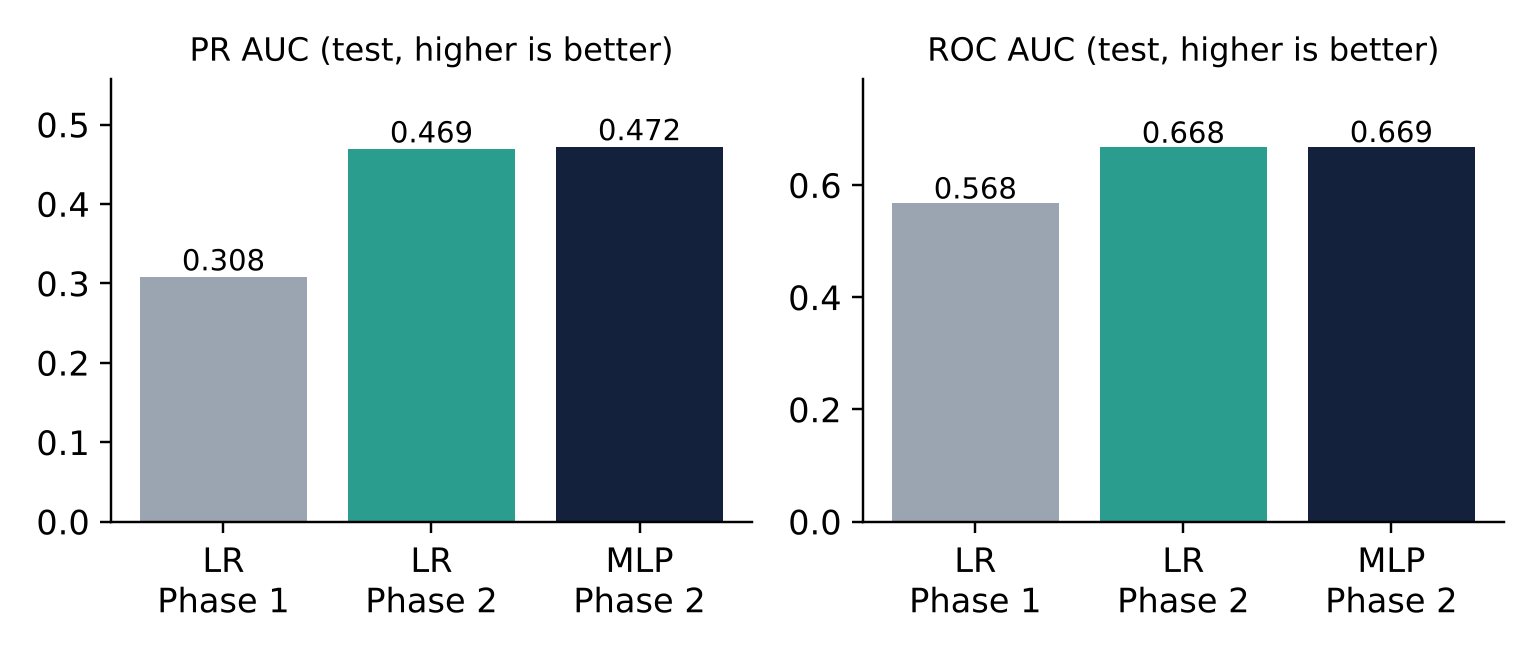
\includegraphics[width=\columnwidth]{fig/main_results.png}
\caption{Test PR~AUC and ROC~AUC. The no-skill PR~AUC equals the test delay rate, 0.267.}
\label{fig:main}
\end{figure}

\begin{figure}[t]
\centering
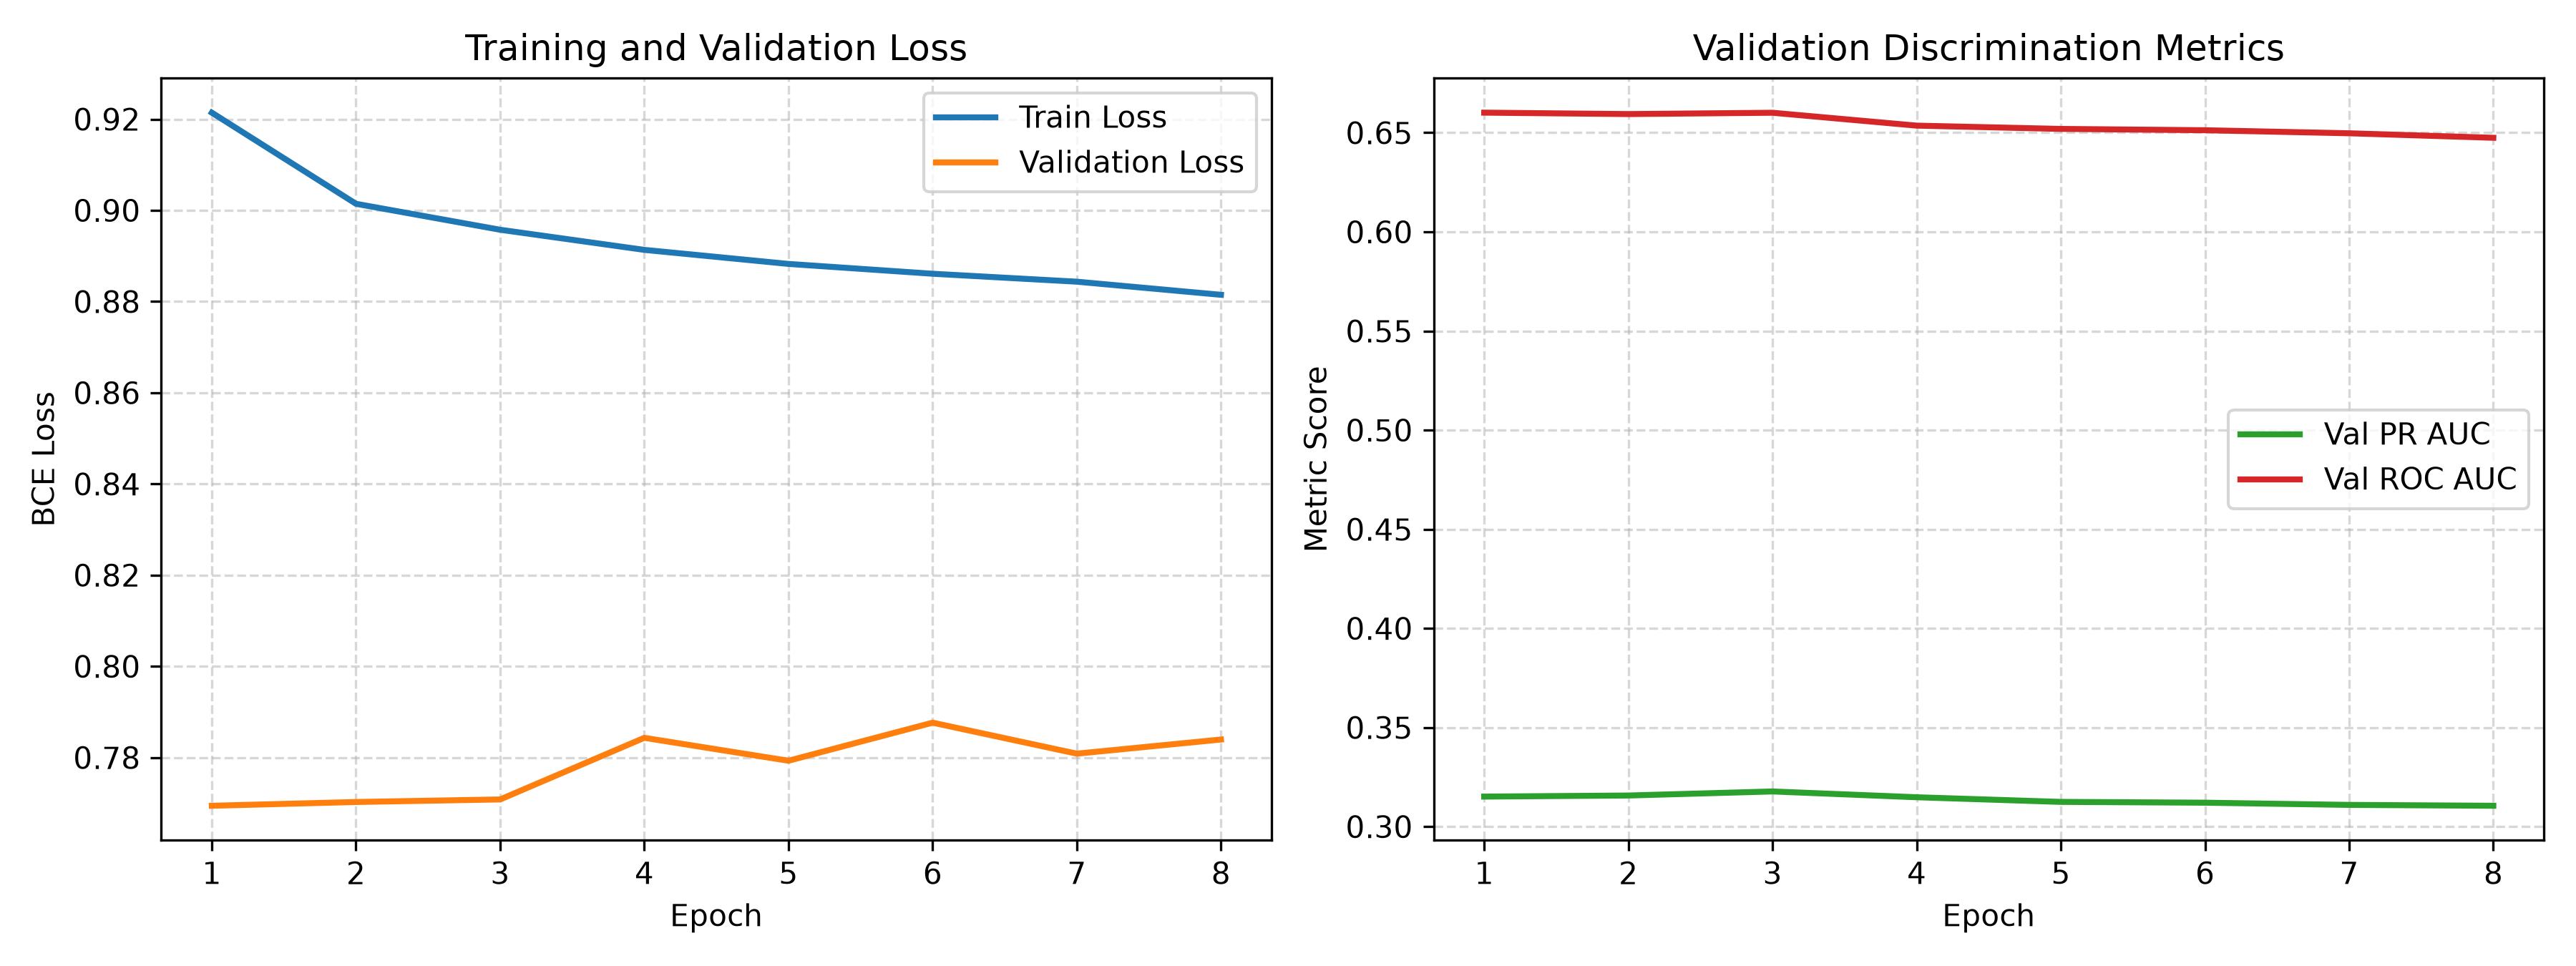
\includegraphics[width=\columnwidth]{fig/training_curves.png}
\caption{MLP training. Validation loss is lowest at epoch 2--3 and then rises while training loss keeps falling, so early stopping selects epoch 3.}
\label{fig:curves}
\end{figure}

Fig.~\ref{fig:curves} shows why early stopping matters: after epoch 3 the network starts to fit the training period more than the validation period. The validation PR~AUC (0.318) is lower than the test PR~AUC because the validation delay rate is much lower (15.4\%), not because of a bug.

\subsection{Ablation studies}
Table~\ref{tab:abl} and Fig.~\ref{fig:abl} show one-factor-at-a-time changes with the same split and seed.

\begin{table}[t]
\caption{Ablations (test set, MLP unless stated)}
\label{tab:abl}
\centering
\small
\setlength{\tabcolsep}{4pt}
\begin{tabular}{llcc}
\toprule
Group & Variant & PR AUC & ROC AUC\\
\midrule
Default & Embeddings, history, dropout 0.3 & 0.4725 & 0.6690\\
\midrule
A & One-hot (no embeddings) & 0.4803 & 0.6771\\
B & No history features & 0.3239 & 0.5889\\
C & Dropout 0.0 & 0.4794 & 0.6768\\
C & Dropout 0.2 & 0.4795 & 0.6770\\
C & Dropout 0.5 & 0.4783 & 0.6744\\
D & Weight decay 0 & 0.4721 & 0.6685\\
D & Weight decay $10^{-3}$ & 0.4718 & 0.6682\\
E & Embedding sizes (2,2,4) & 0.4699 & 0.6697\\
E & Embedding sizes (8,6,16) & 0.4803 & 0.6803\\
F & No class weight & 0.4741 & 0.6701\\
\bottomrule
\end{tabular}
\end{table}

\begin{figure}[t]
\centering
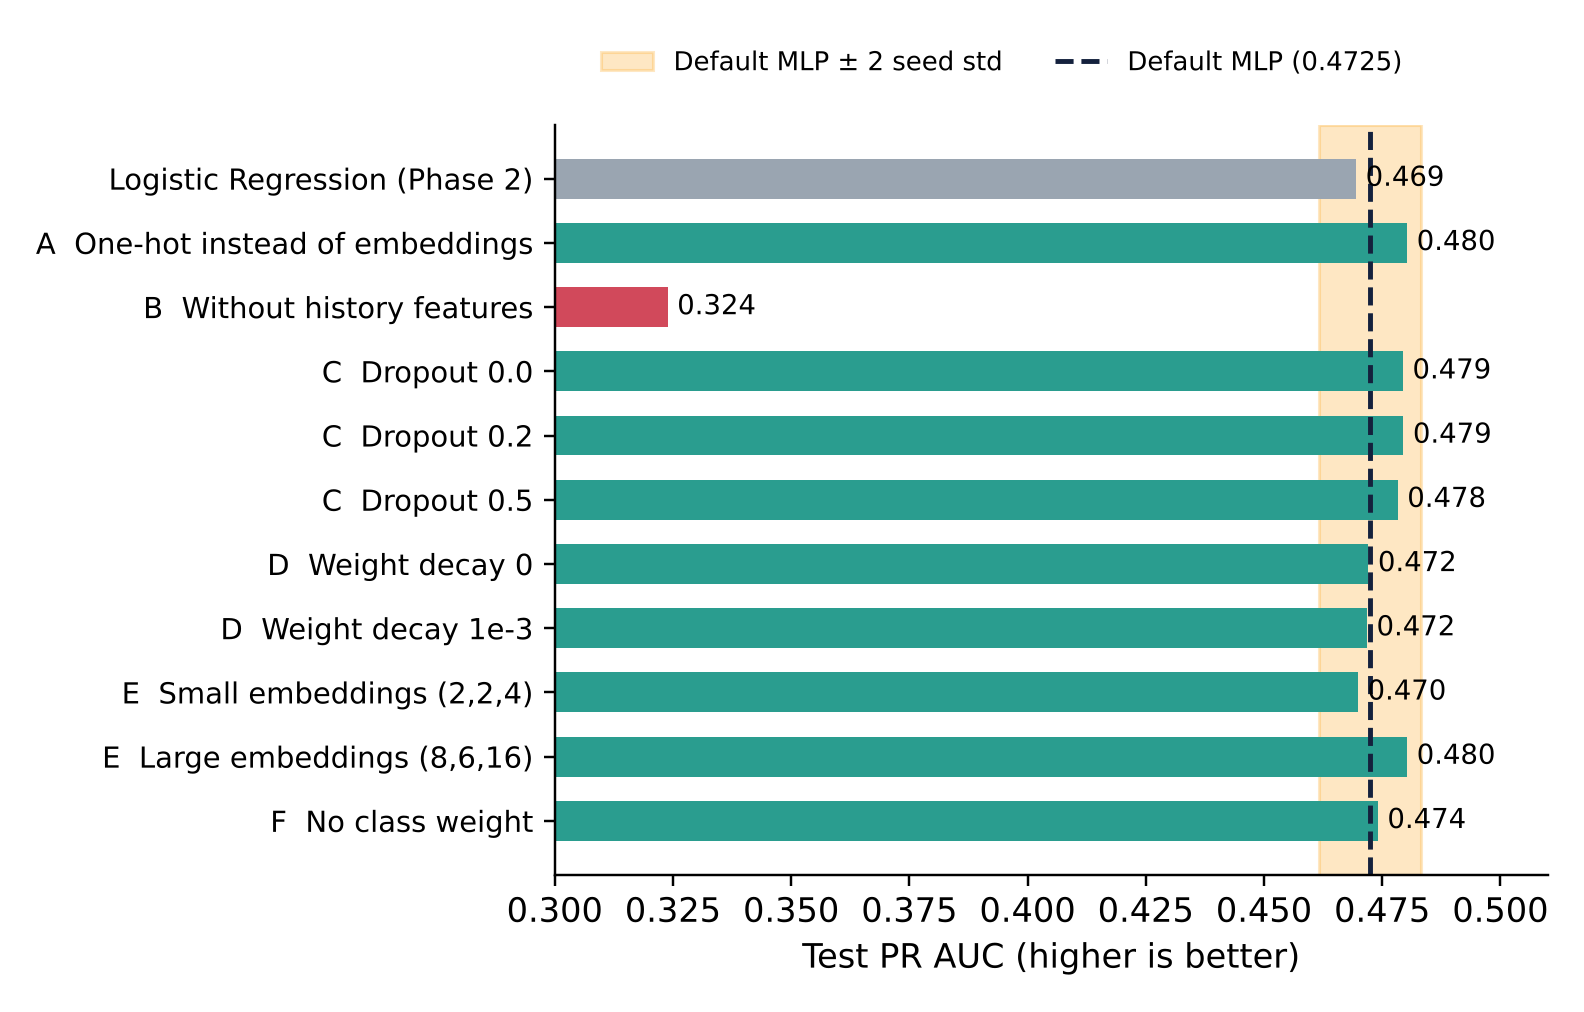
\includegraphics[width=\columnwidth]{fig/ablation_chart.png}
\caption{Ablation results. The shaded band is the default MLP $\pm$ two seed standard deviations; only removing the history features falls clearly outside it.}
\label{fig:abl}
\end{figure}

\emph{History features} are the only factor with a clear effect: removing them lowers PR~AUC by 0.149 and ROC~AUC by 0.080. Every other change is at most 0.008 in PR~AUC, below two seed standard deviations (0.011), so we treat them as noise. In particular, \emph{embeddings did not beat one-hot encoding} (0.4725 vs.\ 0.4803, a difference of 1.4 standard deviations in the wrong direction for embeddings). This is plausible: there are only 16 carriers, 3 origins and about 100 destinations, so one-hot encoding already has enough data per category. Weight decay has no visible effect because training stops after a few epochs with a 14k-parameter network. Class weighting does not change the ranking but changes the probabilities: without it the threshold chosen on validation is 0.24 instead of 0.47 and the Brier score is worse (0.201 vs.\ 0.179); we did not investigate this further. Because ablation runs retrain the model, the default row (0.4725) differs by 0.0002 from the saved model (0.4723) used elsewhere.

\subsection{Calibration and operating point}
\label{sec:calib}
Table~\ref{tab:cal} and Fig.~\ref{fig:rel} give the calibration results on the test set. The raw probabilities are already reasonable (ECE 0.031 for logistic regression, 0.041 for the MLP). Calibration fitted on validation \emph{increases} the error: temperature scaling learns $T=0.570$ and raises the MLP's ECE to 0.072; Platt scaling raises it to 0.117 (MLP) and 0.129 (logistic regression).

\begin{table}[t]
\caption{Calibration on the test set}
\label{tab:cal}
\centering
\small
\setlength{\tabcolsep}{3.5pt}
\begin{tabular}{llcccc}
\toprule
Model & Method & ECE & Brier & PR AUC & ROC AUC\\
\midrule
LR & Raw & 0.031 & 0.179 & 0.470 & 0.668\\
LR & Platt & 0.129 & 0.196 & 0.470 & 0.668\\
MLP & Raw & 0.041 & 0.179 & 0.472 & 0.669\\
MLP & Temp. & 0.072 & 0.184 & 0.472 & 0.669\\
MLP & Platt & 0.117 & 0.193 & 0.472 & 0.669\\
\bottomrule
\end{tabular}
\end{table}

\begin{figure*}[t]
\centering
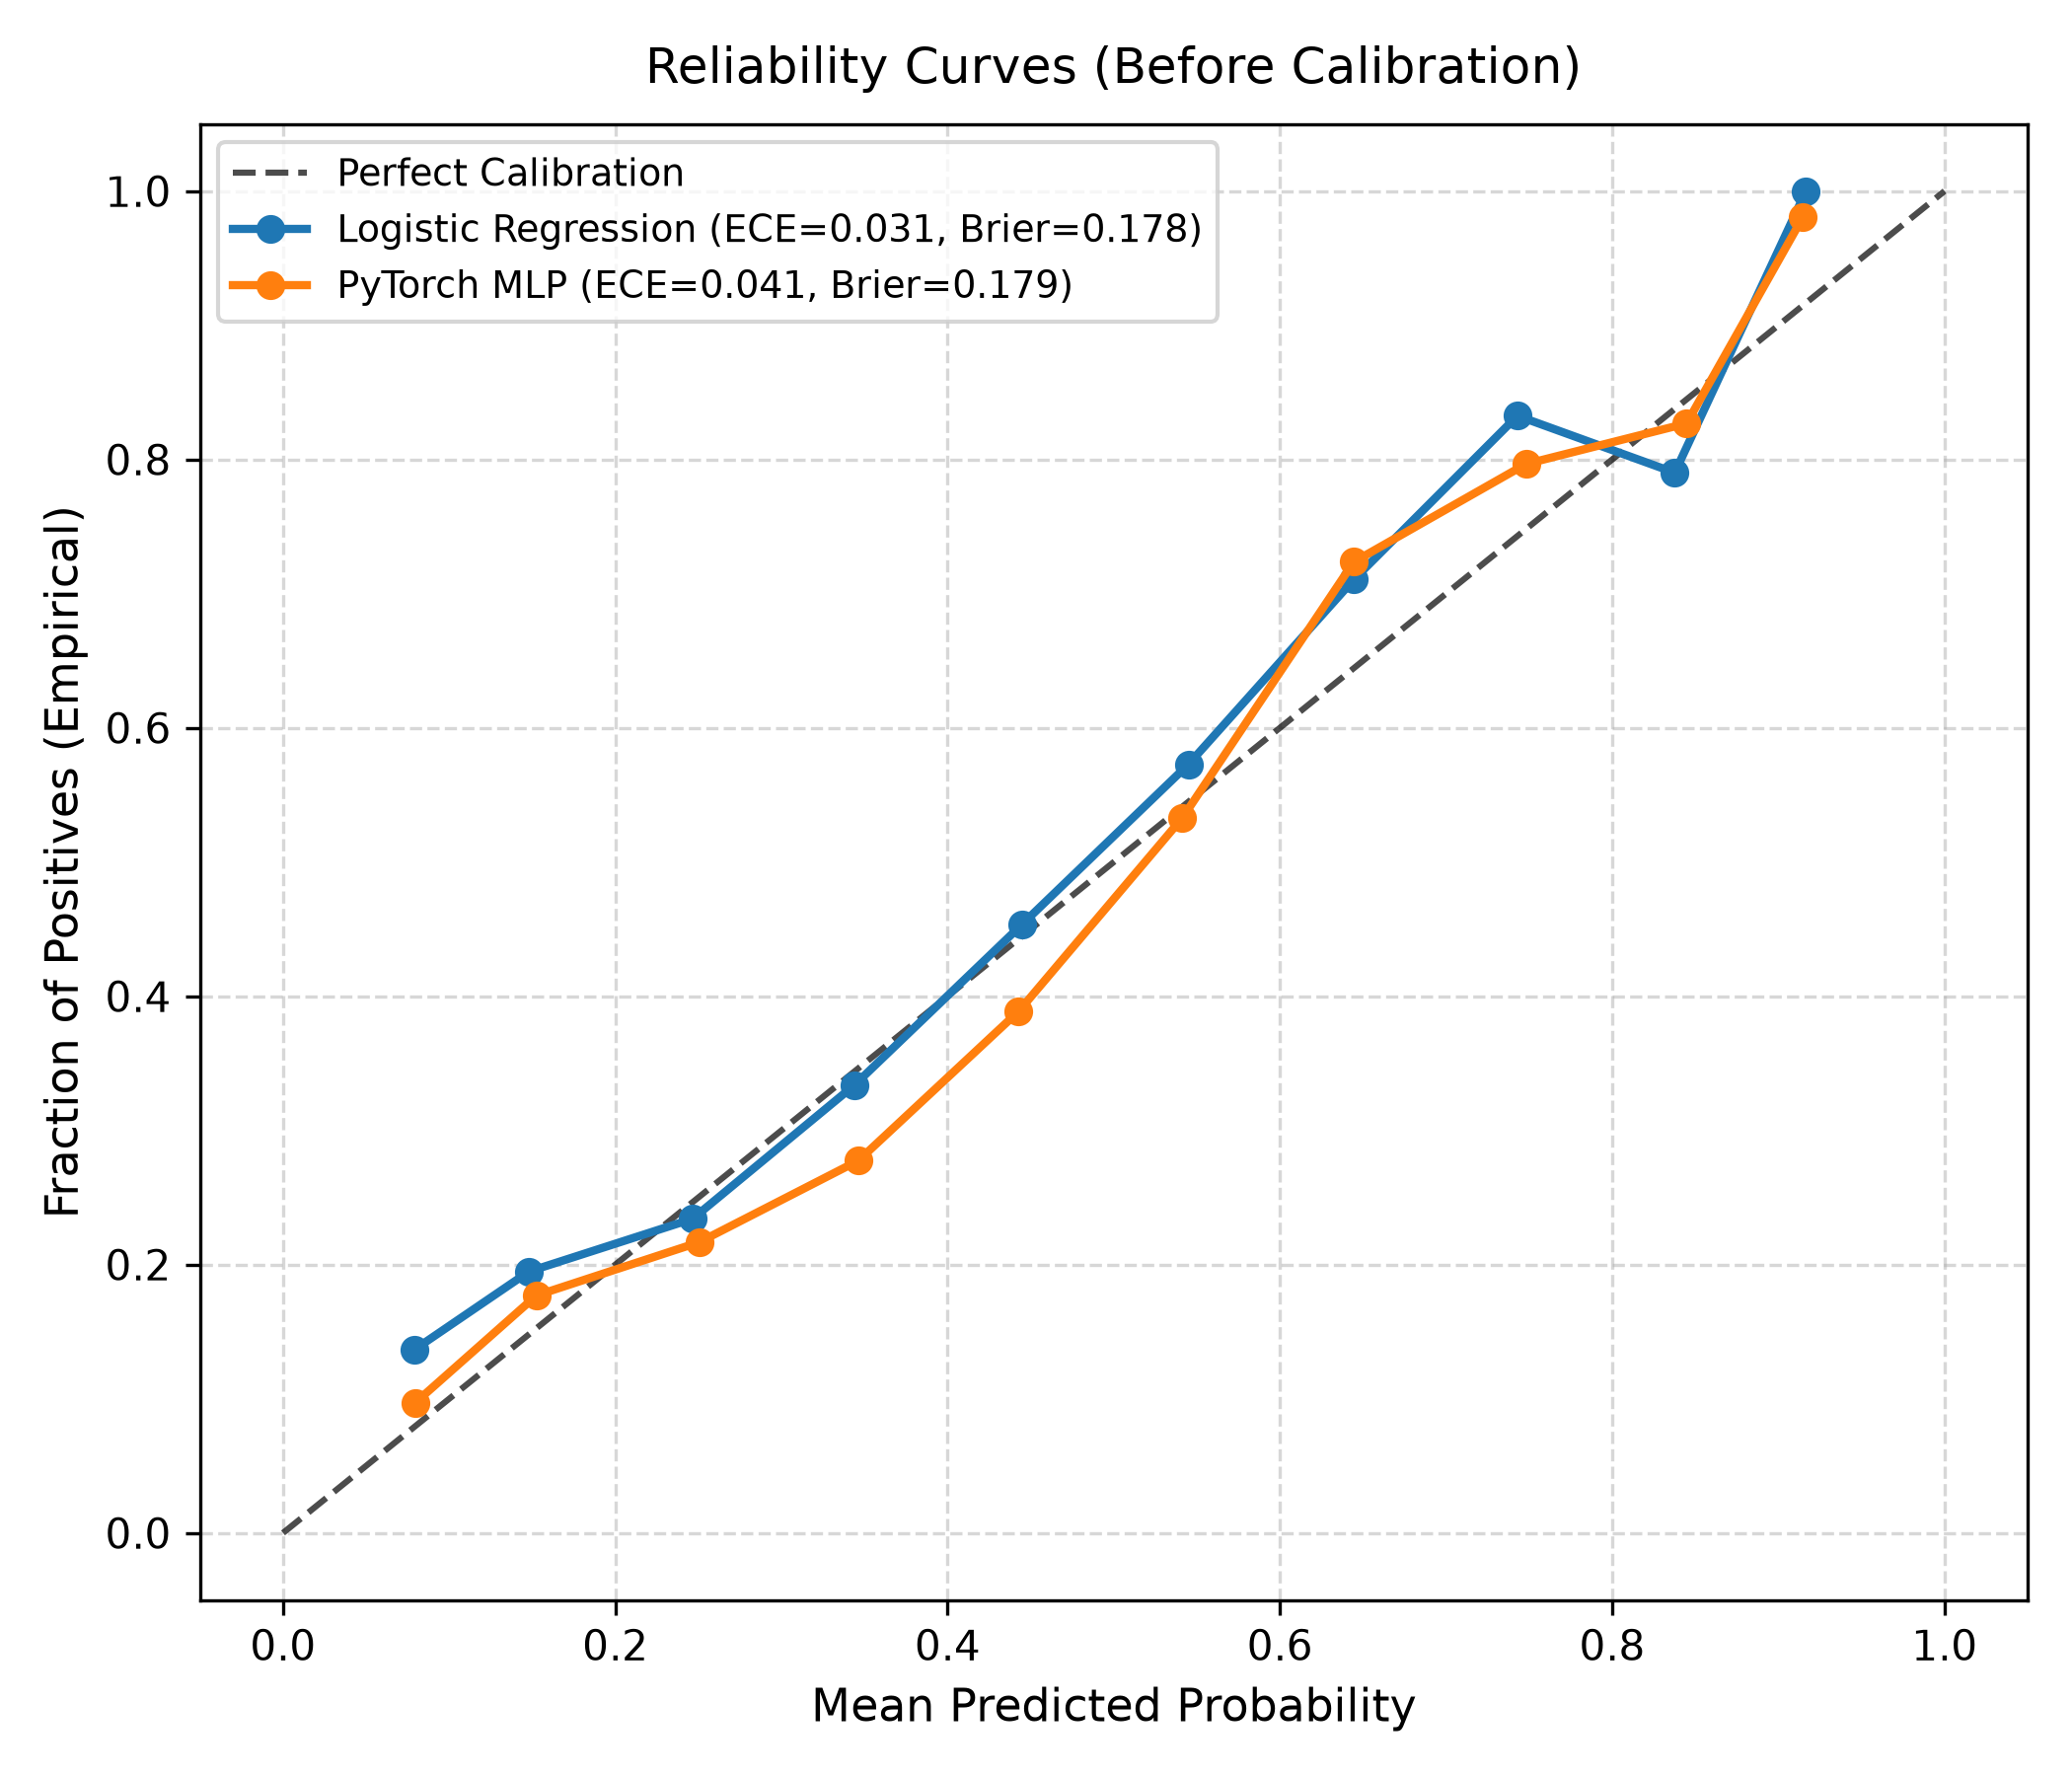
\includegraphics[width=0.40\textwidth]{fig/reliability_before.png}\hspace{0.04\textwidth}
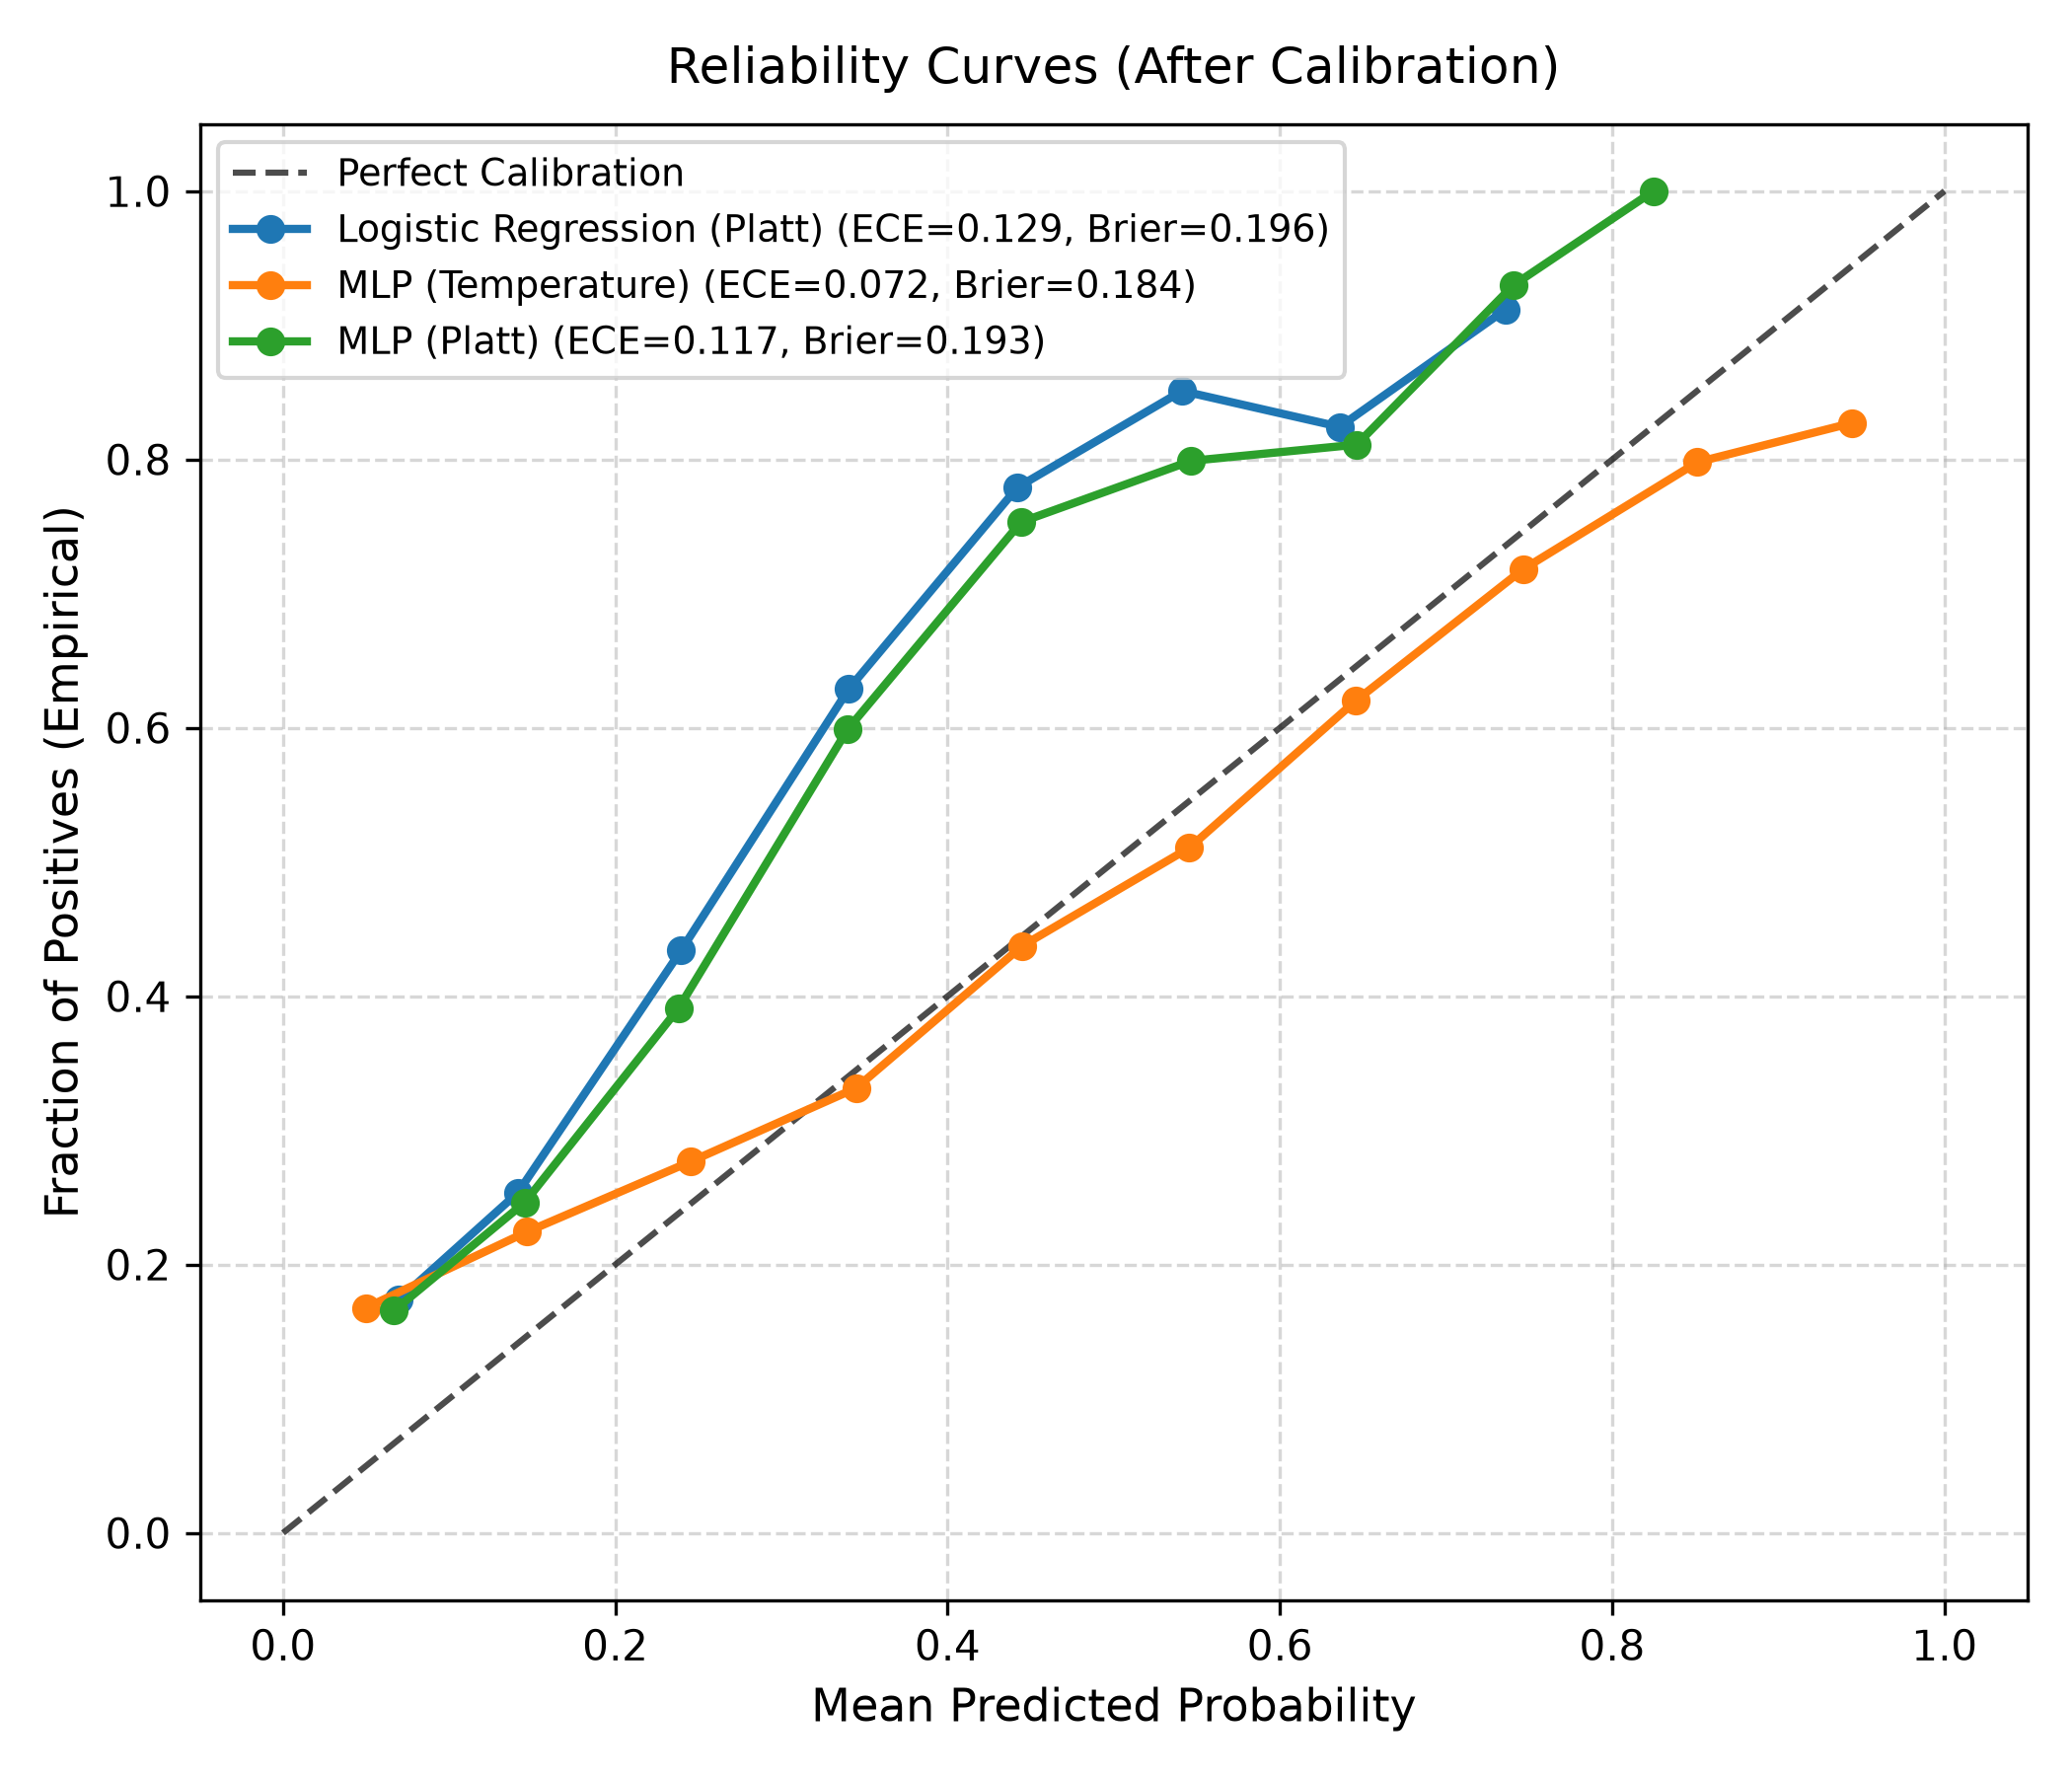
\includegraphics[width=0.40\textwidth]{fig/reliability_after.png}
\caption{Reliability curves on the test set. Left: raw probabilities. Right: after calibration fitted on the validation set. Points above the diagonal mean that real delays are more frequent than predicted.}
\label{fig:rel}
\end{figure*}

The reason is dataset shift. On validation the models predict a mean delay probability of 0.275 (logistic regression) and 0.300 (MLP), but the real delay rate is 0.154; on test the means are 0.245 and 0.290 against a real rate of 0.267. A correction learned on validation therefore tries to lower the probabilities, but the test period needs no such correction. This agrees with the finding that calibration degrades under shift \cite{ovadia}. It also shows that temperature scaling, which only changes confidence and not the average level, cannot repair a base-rate change.

\begin{table}[t]
\caption{Operating points (validation threshold, precision target 0.40) and maximum test recall at minimum precision}
\label{tab:op}
\centering
\small
\setlength{\tabcolsep}{3.5pt}
\begin{tabular}{lccccc}
\toprule
Model & Thr. & Prec. & Rec. & R@P$\ge$.3 & R@P$\ge$.4 \\
\midrule
LR & 0.484 & 0.645 & 0.183 & 0.867 & 0.544\\
MLP & 0.471 & 0.604 & 0.230 & 0.885 & 0.533\\
\bottomrule
\end{tabular}
\end{table}

Table~\ref{tab:op} shows that the validation threshold, aimed at precision 0.40, gives test precision of about 0.60--0.65, because the test period has more delays. At minimum precision 0.50 the maximum recalls are 0.357 (logistic regression) and 0.346 (MLP). The two models are again very close. The PR curves of both models are almost identical (Fig.~\ref{fig:pr}).

\begin{figure}[t]
\centering
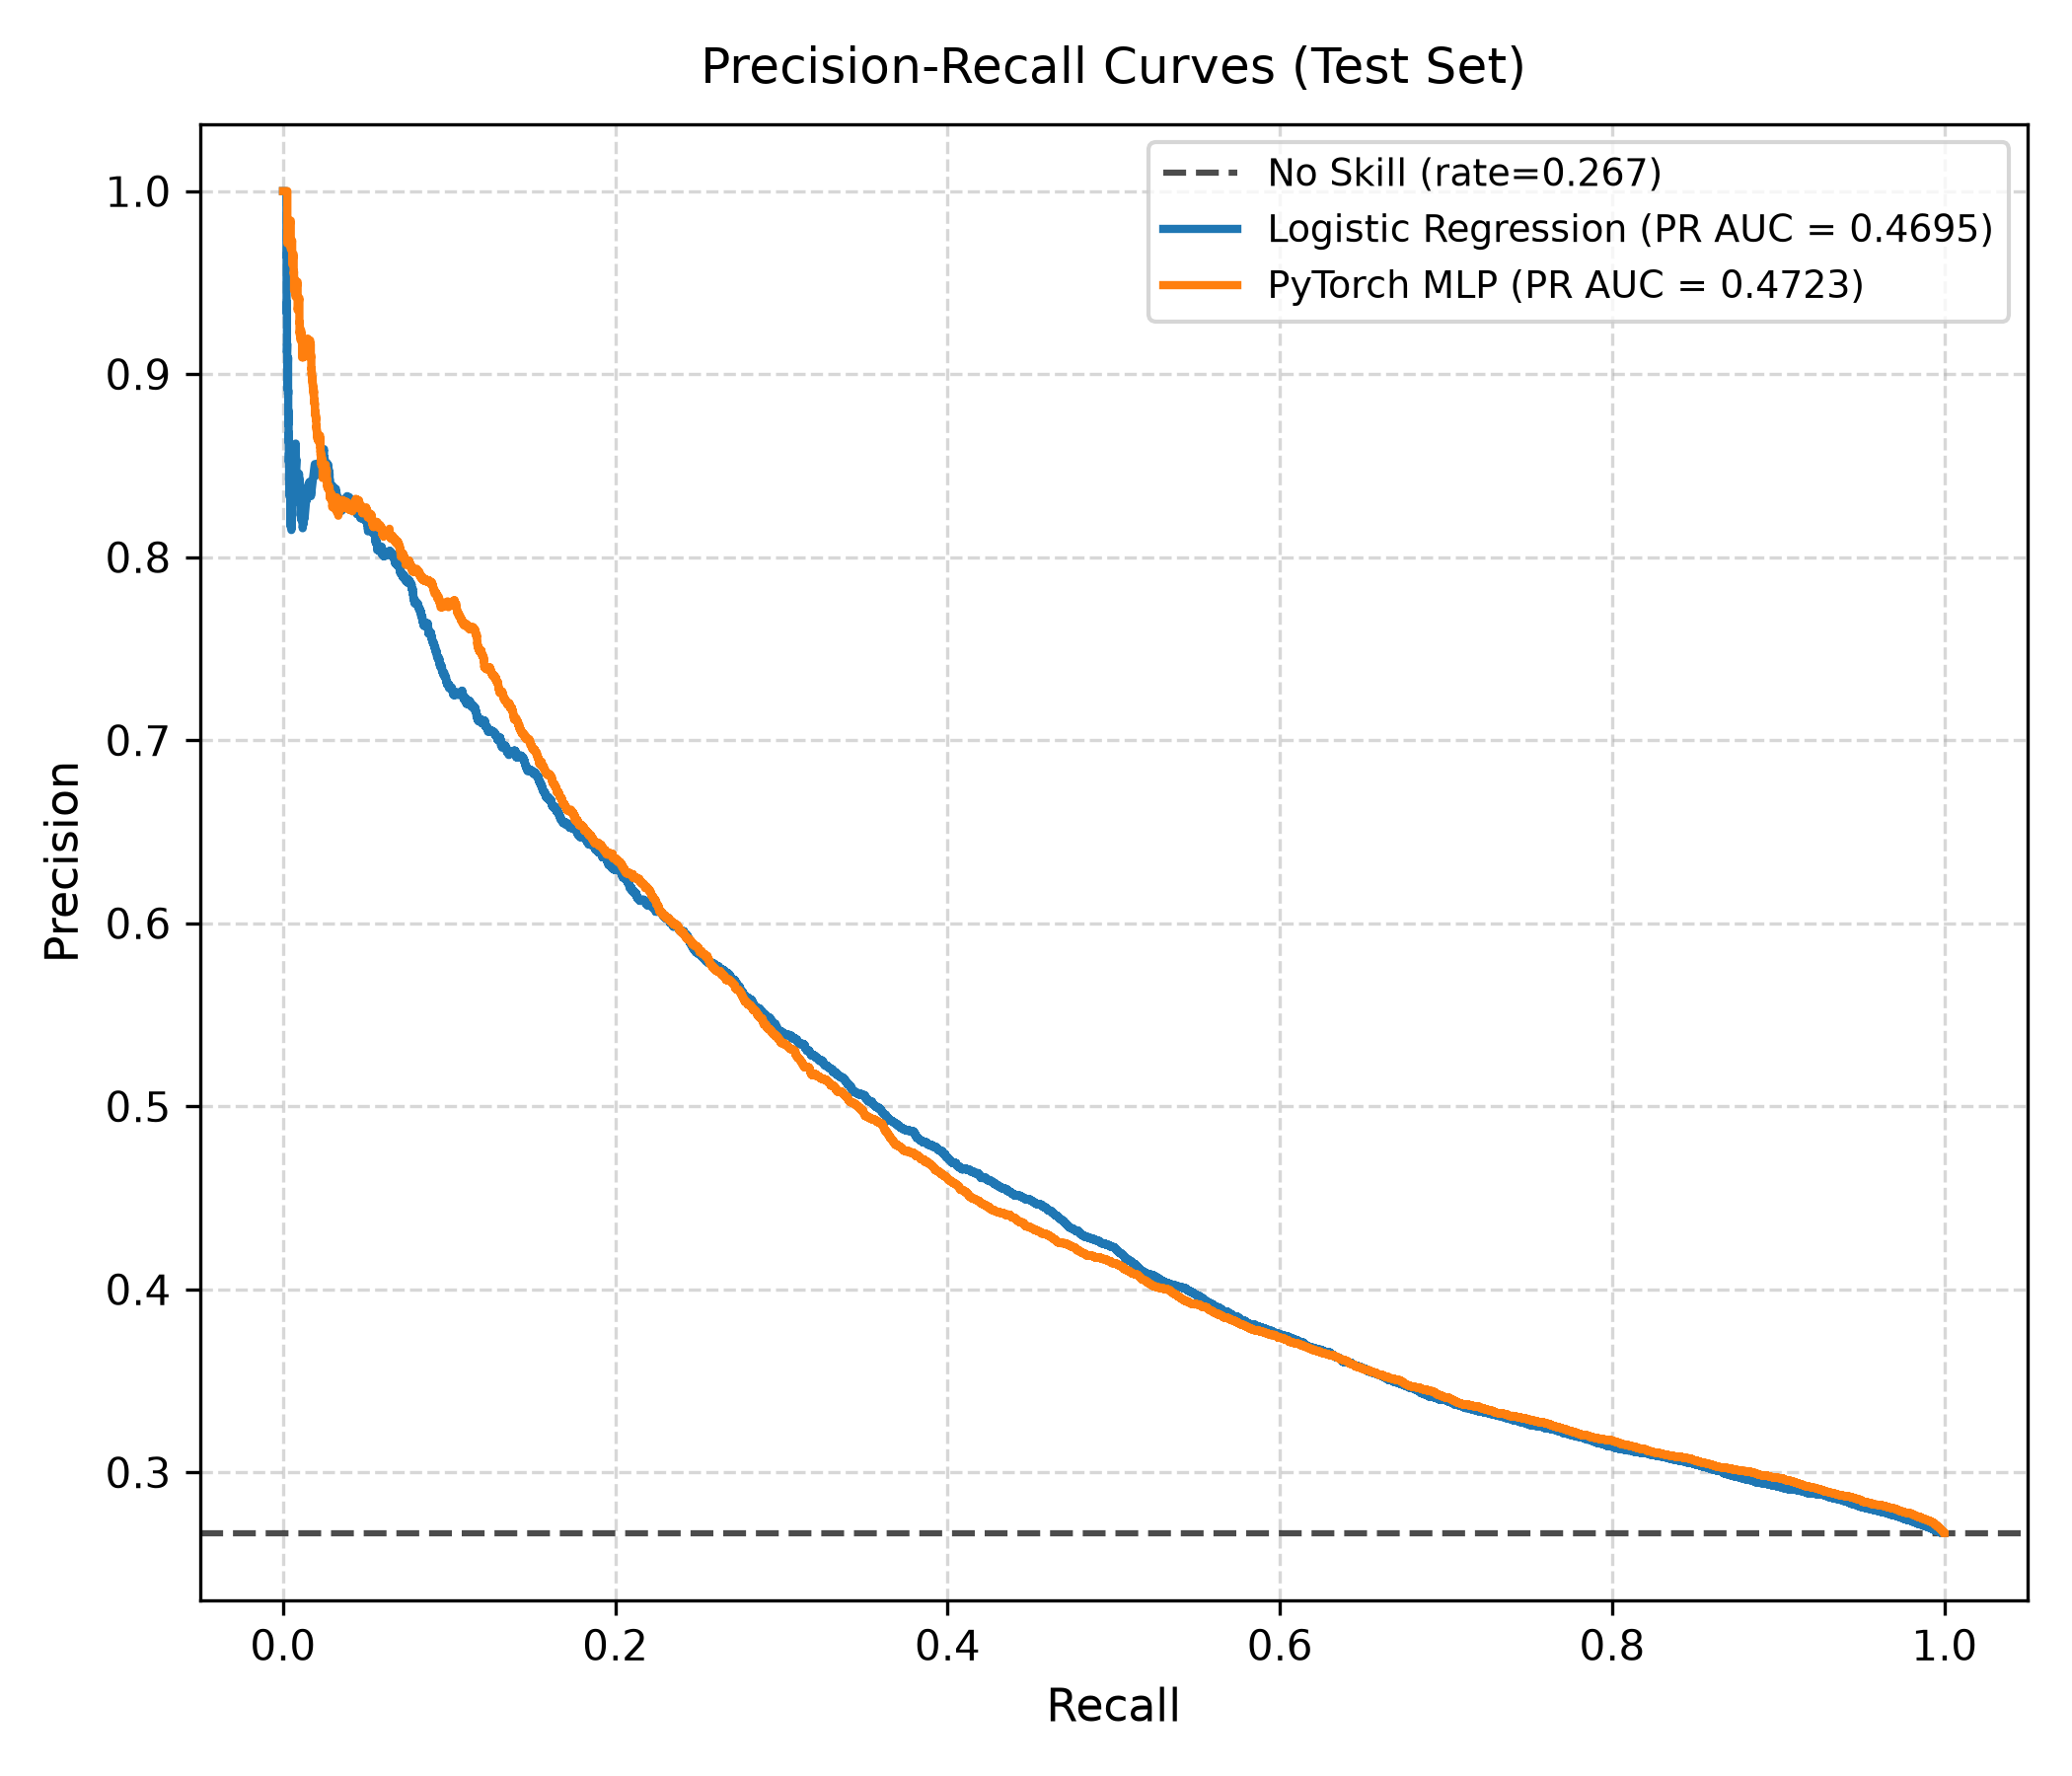
\includegraphics[width=0.92\columnwidth]{fig/pr_curves.png}
\caption{Test precision--recall curves.}
\label{fig:pr}
\end{figure}

\subsection{Offline rescheduling what-if}
\label{sec:resched}
\textbf{Assumptions.} (1) The temperature-scaled MLP output is the true delay probability (Table~\ref{tab:cal} shows this is only approximate). (2) Moves stay on the same day within $\pm$2 hours and between 06:00 and 22:00. (3) Only the hour features change; history and congestion features of the new slot are not recomputed. (4) A move must reduce the risk by more than a penalty $\delta$. (5) At most five moved flights are added per airport-hour. (6) The model's hour effect is treated as causal, which is the weakest assumption. (7) Crews, gates, aircraft rotations and passengers are not modelled. The result is an expected value on past data, not an operational recommendation.

With $\tau=0.40$ and $\delta=0.05$, 6,454 of the 49,102 test flights are flagged and 2,280 (35.3\%) are moved. Their mean risk falls from 0.545 to 0.467, which avoids 179 expected delays: 14.4\% of the risk of the moved flights, but only 1.8\% of the 10,070 expected delays in the test set. Across six settings (Table~\ref{tab:resched}) the benefit ranges from 100 to 242 expected delays (1.0--2.4\%); a lower penalty or threshold moves more flights and gains more.

\begin{table}[t]
\caption{Rescheduling sensitivity (test set)}
\label{tab:resched}
\centering
\small
\setlength{\tabcolsep}{4pt}
\begin{tabular}{ccrrrr}
\toprule
$\tau$ & $\delta$ & Flagged & Moved & Avoided & Risk cut\\
\midrule
0.35 & 0.03 & 8,478 & 3,886 & 242.3 & 12.7\%\\
0.35 & 0.08 & 8,478 & 1,207 & 122.9 & 18.2\%\\
0.40 & 0.03 & 6,454 & 3,074 & 202.9 & 12.3\%\\
0.40 & 0.08 & 6,454 & 1,086 & 112.3 & 17.7\%\\
0.45 & 0.03 & 4,939 & 2,365 & 164.9 & 11.9\%\\
0.45 & 0.08 & 4,939 & 956 & 100.6 & 17.2\%\\
\bottomrule
\end{tabular}
\end{table}

\begin{figure}[t]
\centering
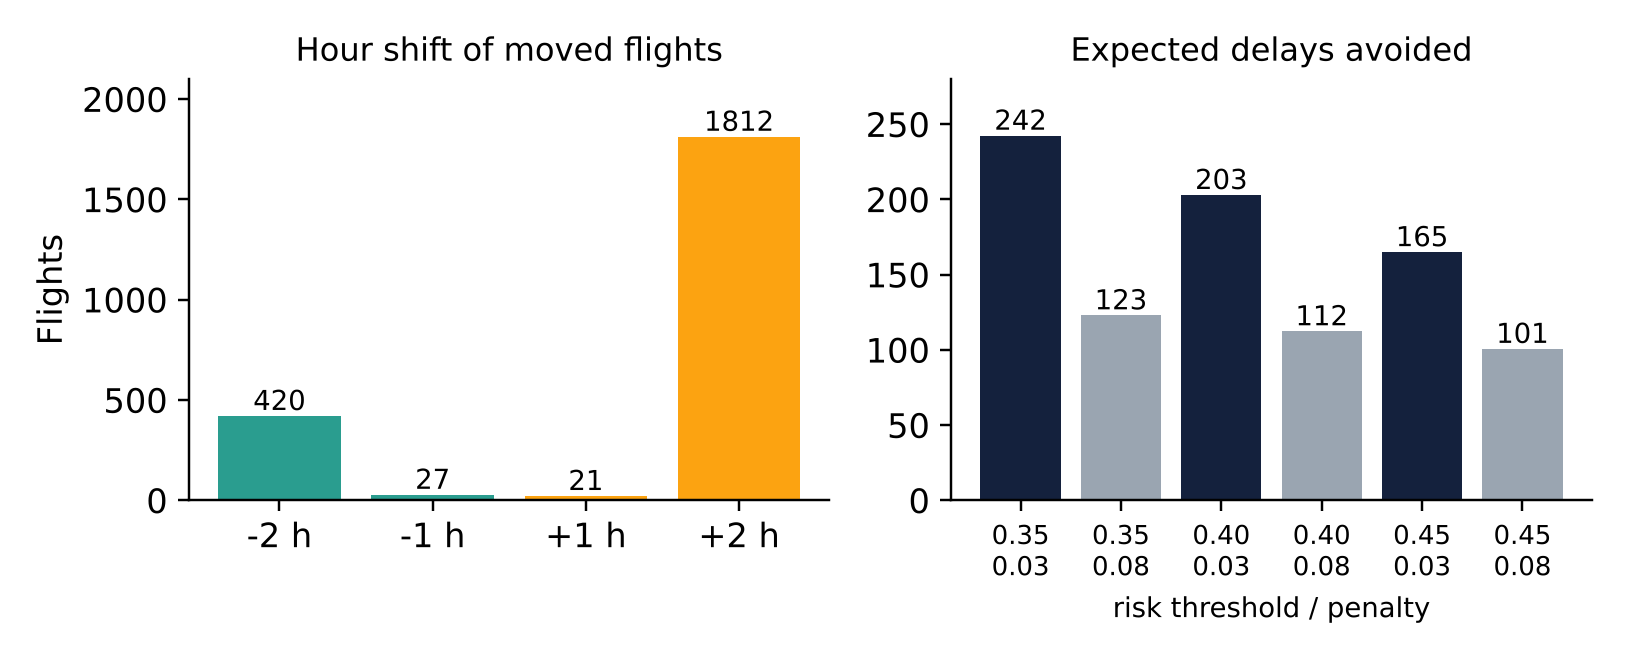
\includegraphics[width=\columnwidth]{fig/resched_chart.png}
\caption{Left: hour shift of the 2,280 moved flights ($\tau=0.40$, $\delta=0.05$). Right: expected delays avoided in the sensitivity study.}
\label{fig:resched}
\end{figure}

A notable pattern is that 80\% of the moves are \emph{later} (1,833 flights moved by $+1$ or $+2$ hours, 447 earlier; Fig.~\ref{fig:resched}). This reflects the hour pattern the model learned, and we did not investigate why. Because assumption (6) is not verified, the gains should be read as an upper-bound style illustration, not as a promise.

\section{Discussion}
\textbf{What worked.} Past-only history features about recent delays at the origin airport improved every model, in line with earlier work on delay state \cite{rebollo}. The leakage tests, the chronological split and the use of a validation set for all choices give us confidence that the improvement is not caused by leakage.

\textbf{What did not.} The neural network did not clearly beat logistic regression, embeddings did not beat one-hot encoding, and regularisation settings made no measurable difference. This matches the general finding that deep learning has no automatic advantage on tabular data \cite{grinsztajn,shwartz}. Calibration fixes fitted on validation made the test calibration worse because of the base-rate shift. We think these are honest and useful findings, and they were only visible because we measured seed noise and used separate validation and test periods.

\textbf{Limitations.} (1) One year of data from three airports: seasonal effects cannot be separated from the shift, and the validation period is unrepresentative. (2) No weather, no aircraft-rotation or network features, although weather is a main driver of delays \cite{choi}. (3) Seed noise (std 0.005) is larger than most ablation effects, and five seeds is a small sample. (4) An early internal run of XGBoost on the same history features reached a PR~AUC of 0.407, below both models here; it was dropped from the final Phase~2 pipeline for stability reasons, so we make no claim about gradient boosting with these features. (5) The rescheduling study depends on a causal reading of the hour effect and ignores real operational constraints. (6) No hybrid or temporal model was built.

\textbf{Future work.} Add weather and previous-flight-of-the-same-aircraft features; use multi-year data so that calibration can be fitted on a period closer to the test period; try a recency-weighted calibration set or a base-rate (intercept) correction; compare with gradient boosting under the same protocol; and test a temporal model only if the flight history is correctly ordered.

\section{Conclusion}
Under a strict two-hour-ahead, leakage-tested, chronological protocol, recent-delay history features raise PR~AUC from 0.308 to about 0.47. A compact embedding MLP matches, but does not significantly beat, logistic regression. Ablations with a seed-noise estimate show that the data matter more than the architecture, and calibration under dataset shift needs more care than a single validation-fitted correction. An offline rescheduling study shows a small expected benefit under strong assumptions.

\begin{thebibliography}{99}
\bibitem{carvalho} L. Carvalho \emph{et al.}, ``On the relevance of data science for flight delay research: A systematic review,'' \emph{Transport Reviews}, 2021, doi: 10.1080/01441647.2020.1861123.
\bibitem{rebollo} J. J. Rebollo and H. Balakrishnan, ``Characterization and prediction of air traffic delays,'' \emph{Transp. Res. C, Emerg. Technol.}, vol. 44, pp. 231--241, 2014.
\bibitem{choi} S. Choi, Y. J. Kim, S. Briceno, and D. Mavris, ``Prediction of weather-induced airline delays based on machine learning algorithms,'' in \emph{Proc. IEEE/AIAA 35th Digit. Avionics Syst. Conf. (DASC)}, 2016, pp. 1--6.
\bibitem{kim} Y. J. Kim, S. Choi, S. Briceno, and D. Mavris, ``A deep learning approach to flight delay prediction,'' in \emph{Proc. IEEE/AIAA 35th Digit. Avionics Syst. Conf. (DASC)}, 2016, pp. 1--6.
\bibitem{yu} B. Yu, Z. Guo, S. Arisian, H. Wang, and G. Chen, ``Flight delay prediction for commercial air transport: A deep learning approach,'' \emph{Transp. Res. E, Logist. Transp. Rev.}, vol. 125, pp. 203--221, 2019.
\bibitem{yazdi} M. F. Yazdi, S. R. Kamel, S. J. M. Chabok, and M. Kheirabadi, ``Flight delay prediction based on deep learning and Levenberg--Marquart algorithm,'' \emph{J. Big Data}, vol. 7, art. 106, 2020.
\bibitem{guoberk} C. Guo and F. Berkhahn, ``Entity embeddings of categorical variables,'' arXiv:1604.06737, 2016.
\bibitem{grinsztajn} L. Grinsztajn, E. Oyallon, and G. Varoquaux, ``Why do tree-based models still outperform deep learning on typical tabular data?'' in \emph{Proc. NeurIPS Datasets and Benchmarks Track}, 2022.
\bibitem{shwartz} R. Shwartz-Ziv and A. Armon, ``Tabular data: Deep learning is not all you need,'' \emph{Inf. Fusion}, vol. 81, pp. 84--90, 2022.
\bibitem{srivastava} N. Srivastava, G. Hinton, A. Krizhevsky, I. Sutskever, and R. Salakhutdinov, ``Dropout: A simple way to prevent neural networks from overfitting,'' \emph{J. Mach. Learn. Res.}, vol. 15, pp. 1929--1958, 2014.
\bibitem{ioffe} S. Ioffe and C. Szegedy, ``Batch normalization: Accelerating deep network training by reducing internal covariate shift,'' in \emph{Proc. ICML}, 2015, pp. 448--456.
\bibitem{adamw} I. Loshchilov and F. Hutter, ``Decoupled weight decay regularization,'' in \emph{Proc. ICLR}, 2019.
\bibitem{prechelt} L. Prechelt, ``Early stopping---but when?'' in \emph{Neural Networks: Tricks of the Trade}. Berlin, Germany: Springer, 1998, pp. 55--69.
\bibitem{johnson} J. M. Johnson and T. M. Khoshgoftaar, ``Survey on deep learning with class imbalance,'' \emph{J. Big Data}, vol. 6, art. 27, 2019.
\bibitem{davis} J. Davis and M. Goadrich, ``The relationship between precision-recall and ROC curves,'' in \emph{Proc. ICML}, 2006, pp. 233--240.
\bibitem{saito} T. Saito and M. Rehmsmeier, ``The precision-recall plot is more informative than the ROC plot when evaluating binary classifiers on imbalanced datasets,'' \emph{PLoS ONE}, vol. 10, no. 3, e0118432, 2015.
\bibitem{platt} J. C. Platt, ``Probabilistic outputs for support vector machines and comparisons to regularized likelihood methods,'' in \emph{Advances in Large Margin Classifiers}. Cambridge, MA, USA: MIT Press, 1999, pp. 61--74.
\bibitem{nm} A. Niculescu-Mizil and R. Caruana, ``Predicting good probabilities with supervised learning,'' in \emph{Proc. ICML}, 2005, pp. 625--632.
\bibitem{guo} C. Guo, G. Pleiss, Y. Sun, and K. Q. Weinberger, ``On calibration of modern neural networks,'' in \emph{Proc. ICML}, 2017, pp. 1321--1330.
\bibitem{naeini} M. P. Naeini, G. F. Cooper, and M. Hauskrecht, ``Obtaining well calibrated probabilities using Bayesian binning,'' in \emph{Proc. AAAI}, 2015, pp. 2901--2907.
\bibitem{brier} G. W. Brier, ``Verification of forecasts expressed in terms of probability,'' \emph{Mon. Weather Rev.}, vol. 78, no. 1, pp. 1--3, 1950.
\bibitem{ovadia} Y. Ovadia \emph{et al.}, ``Can you trust your model's uncertainty? Evaluating predictive uncertainty under dataset shift,'' in \emph{Proc. NeurIPS}, 2019.
\bibitem{bts} Bureau of Transportation Statistics, ``Airline on-time performance data,'' U.S. Department of Transportation. [Online]. Available: https://www.transtats.bts.gov
\bibitem{wick} H. Wickham, ``nycflights13: Flights that departed NYC in 2013,'' R package, CRAN.
\bibitem{paszke} A. Paszke \emph{et al.}, ``PyTorch: An imperative style, high-performance deep learning library,'' in \emph{Proc. NeurIPS}, 2019.
\bibitem{sklearn} F. Pedregosa \emph{et al.}, ``Scikit-learn: Machine learning in Python,'' \emph{J. Mach. Learn. Res.}, vol. 12, pp. 2825--2830, 2011.
\end{thebibliography}

\end{document}
